\newpage
\chapter{Anhang} 

\section{Wörter zählen und Top 20 Ranking ausgeben}\label{code:wordcount}


\lstinputlisting[language=Java, firstline=26, lastline=54]{./programmierung/spark/src/main/java/spark/SeminararbeitTop20Woerter.java}

%\begin{figure}[h]
 % \centering
  %\fbox{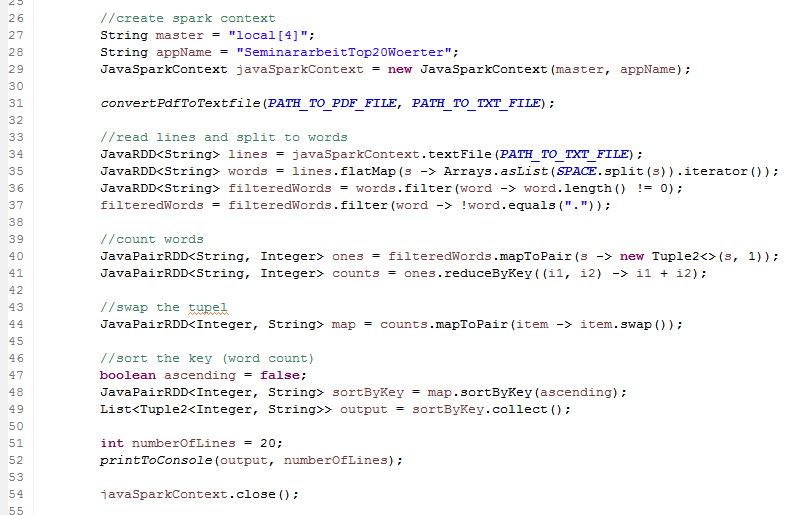
\includegraphics[width=140mm]{./bilder/listing_top20_1.PNG}}  
%\end{figure}

\newpage
\section{Beispielimplementierung für den Verbund mehrerer Spark Komponenten}
\subsection{Einlesen der Daten}\label{code:verbund_1}

\lstinputlisting[language=Java, firstline=24, lastline=41]{./programmierung/spark/src/main/java/spark/AnalyseEmployees.java}
\vspace{0.7cm}
%\begin{figure}[h]
 % \centering
  %\fbox{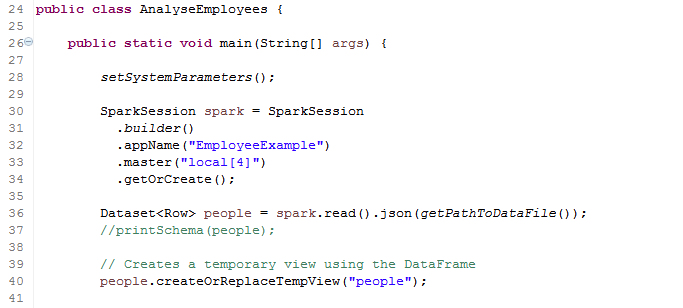
\includegraphics[width=140mm]{./bilder/code_verbund_1_1.PNG}}
%\end{figure}

%\newpage
\subsection{Maschinelles Lernen}\label{code:verbund_2}
\lstinputlisting[language=Java, firstline=42, lastline=72]{./programmierung/spark/src/main/java/spark/AnalyseEmployees.java} 

%\begin{figure}[ht]
 % \centering
  %\fbox{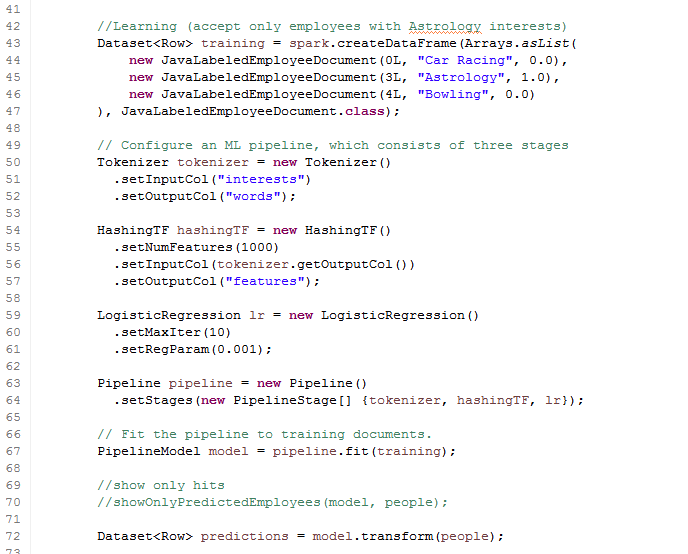
\includegraphics[width=140mm]{./bilder/code_verbund_2_1.PNG}}  
%\end{figure}

\newpage
\subsection{MapReduce und Ausgabe}\label{code:verbund_3}
\lstinputlisting[language=Java, firstline=74, lastline=102]{./programmierung/spark/src/main/java/spark/AnalyseEmployees.java} 
%\begin{figure}[h]
 % \centering
  %\fbox{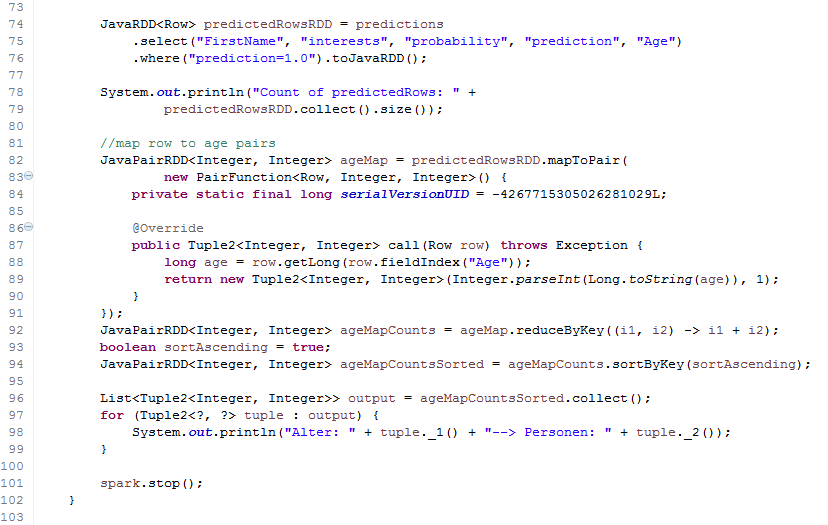
\includegraphics[width=140mm]{./bilder/code_verbund_3_1.PNG}}  
%\end{figure}
\vspace{0.7cm}
\subsection{Ergebnis}\label{code:verbund_4}
\begin{figure}[h]
  \centering
  \fbox{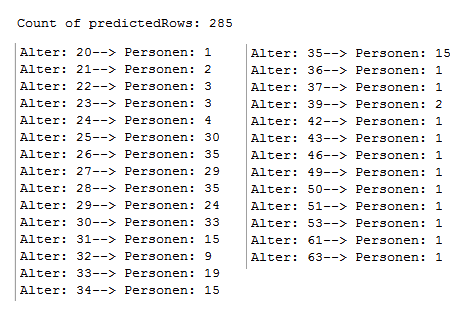
\includegraphics[width=100mm]{./bilder/code_verbund_4.PNG}}  
\end{figure}